% *********************** Це є Розділ 2 ************************************

 %\markright{\underline {\it Розділ 2. Теоретичне рішення проблеми}}

 %\setcounter{chapter}{1}
 \chapter{ТЕОРЕТИЧНЕ ВИРІШЕННЯ ПРОБЛЕМИ}

 
 У цьому розділі розглядається теоретичне підґрунтя розв'язання задачі рендерингу в рамках створення власного графічного рушія. Спочатку описується 
 базовий процес рендерингу геометрії, далі розглядаються моделі BRDF, що визначають фізично коректне відбиття світла від поверхонь, а також методи оптимізації, 
 які забезпечують ефективну роботу системи в реальному часі.

\section{Рендеринг геометрії}
  \setcounter{equation}{0}
 \setcounter{theorem}{0}
 Рендеринг геометрії є фундаментальною складовою комп’ютерної графіки й одночасно однією з найскладніших задач. Безпосереднє математичне описання складних форм (наприклад, анатомії людини) аналітичними функціями практично неможливе, тому використовуються чисельні апроксимації. Найпоширеніший підхід полягає в розбитті поверхні на набір елементарних багатокутників, зазвичай -- трикутників. Така триангуляція дозволяє будь–який многовид наближати довільно точно, регулюючи щільність сітки.

Графічний процесор (GPU) оптимізований під ефективну обробку саме трикутних сіток. Кожен трикутник задається трьома вершинами та відповідними індексами ребер. GPU приймає буфери вершин і індексів, виконує трансформації та проєкцію, а потім передає дані далі в конвеєр -- тобто в pipeline.

\subsection*{Графічний конвеєр і шейдери}
Графічний пайплайн складається з кількох етапів:
\begin{enumerate}
    \item \textbf{Вершинний шейдер (Vertex Shader)} -- застосовує афінні пе\-рет\-во\-рен\-ня до вершин: поворот, масштаб, перенесення та проєкцію у відсічений об’єм.
    \item \textbf{Тесселяція (опціонально)} -- процес динамічного розбиття примітивів (переважно трикутників або чотирикутників), що формують геометрію об'єктів, на менші  з метою підвищення рівня деталізації. 
      
    \item \textbf{Геометричний шейдер (Geometry Shader)} -- може додатково генерувати чи модифікувати примітиви на основі вхідних даних.
    \item \textbf{Растеризація} -- перетворює примітиви (трикутники) у фрагменти (пік\-се\-лі), відсікає ті, що знаходяться поза областю перегляду.
    \item \textbf{Фрагментний (піксельний) шейдер (Fragment / Pixel Shader)} -- обчислює колір кожного фрагмента з урахуванням матеріальних влас\-ти-\-вос\-тей і текстур.
    \item \textbf{Тест глибинності й блендінг} -- вирішує, які фрагменти за\-ли\-шаю\-ть\-ся у фінальному буфері кадру.
\end{enumerate}

\subsection*{Перспективна проєкція та відсікання.}
Для реалізації правдоподібного відтворення сцени необхідно врахувати сприйняття глибинних відстаней людиною. \textit{Перспективна проєкція} формально задається усіченою пірамідою, яку можна визначити матрицею:
\[
P = 
\begin{pmatrix}
\frac{1}{\tan(\tfrac{fov}{2})\,a} & 0 & 0 & 0 \\
0 & \frac{1}{\tan(\tfrac{fov}{2})} & 0 & 0 \\
0 & 0 & \frac{z_\mathrm{far}+z_\mathrm{near}}{z_\mathrm{near}-z_\mathrm{far}} & \frac{2\,z_\mathrm{far}\,z_\mathrm{near}}{z_\mathrm{near}-z_\mathrm{far}} \\
0 & 0 & -1 & 0
\end{pmatrix},
\]
де $fov$ -- кут огляду, $a$ -- аспектне співвідношення екрану, $z_\mathrm{near}$ і $z_\mathrm{far}$ -- межі відсічення. Перспектива забезпечує зменшення розмірів 
віддалених об’єктів і дає змогу відсікати геометрію поза ближня і дальня площини відсікання, що знижує навантаження на конвеєр.

\subsection*{Текстурування і матеріали.}
Окрім геометрії, для реалістичного виг\-ля\-ду необхідно вказати:
\begin{itemize}
    \item \textbf{Колір (Albedo)} -- базова текстура дифузного відбиття.
    \item \textbf{Шорсткість(Roughness) / Металічність(Metalness)} -- парамет\-ри для PBR-моделювання, які відповідають за фізичні властивості матеріалу.
    \item \textbf{Текстурування нормалей(Normal Map)} -- для імітації дрібних нерівностей, за рахунок модифікування нормалі точок поверхні без збільшення полігонів.
\end{itemize}

У піксельному шейдері ці карти комбінуються з параметрами світла та BRDF, щоб отримати остаточний колір пікселя.

\medskip
Таким чином, рендеринг геометрії охоплює низку послідовних етапів: від апроксимації форми трикутниками, через трансформації та відсікання, до текстурування й 
шейдерної обробки, причому на кожному кроці необхідно балансувати між якістю зображення та продуктивністю системи.

\section{Мікрофасетна модель відбиття}
\setcounter{equation}{0}
\setcounter{theorem}{0}

У цьому підрозділі розглядається мікрофасетна модель відбиття світла \linebreak Cook-Tor\-ran\-ce BRDF. Вперше ця модель була запропонована 
в 1982 році у праці Роберта Кука та Кеннета Торренса \cite{cook1982reflectance} як фізично обґрунтована альтернатива емпіричним моделям відбиття, таким як Фонг або Блінн–Фонг.

\subsection{BRDF}\\
\par
Основна ідея BRDF полягає у тому, що поверхня моделюється як сукупність уявних мікрофасетів. Кожна така мікрофасета роз\-гля\-да\-єть\-ся як ідеальне дзеркало. Поведінка макроскопічної поверхні описується статистично 
через розподіл орієнтацій цих мікрофасетів.

\par
Цей підхід дозволяє значно точніше апроксимувати фізичні властивості реальних матеріалів порівняно з класичними моделями, що були раніше поширені в
 рендерінгу у реальному часі. Наприклад, модель Фонга була популярною завдяки своїй обчислювальній простоті. Проте із розвитком обчислювальної техніки 
 галузь комп'ютерної графіки майже повністю перейшла на фізично обґрунтований рендеринг (Physically Based Rendering, PBR), де мікрофасетні моделі відіграють
  ключову роль як в офлайн-рендерінгу, так і в рендерінгу в реальному часі.

\par
На конференції SIGGRAPH 2012 року \cite{Ch6} Брент Берлі, дослідник з \textit{Walt Disney Animation Studios}, запропонував спрощений інтерфейс для
 використання мікрофасетної моделі BRDF. У цьому підході всі параметри нормалізовано до інтервалу $[0;1]$, що суттєво спрощує взаємодію з моделлю. 
Цей підхід відомий як \textit{metallic–roughness workflow} (металево-шорсткий підхід) і нині є де-факто стандартом для опису матеріалів у комп’ютерній графіці.

Модель ґрунтується на двох основних параметрах:
\begin{itemize}
    \item \textbf{Металевість} (\textit{metallic}) -- визначає тип матеріалу: метал (\textit{metallic} = 1) або діелектрик (\textit{metallic} = 0). Метали, 
    такі як золото, срібло чи мідь, мають високу дзеркальну відбивну здатність. Діелектрики (наприклад, пластик, дерево, гума) мають інший характер відбиття світла.
    
    \item \textbf{Шорсткість} (\textit{roughness}) -- описує розсіювання мікрофасетів. Для ідеально гладких поверхонь (наприклад, полірування) \textit{roughness} = 0,
     і всі мікрофасети орієнтовані однаково, що створює дзеркальне відбиття. Із зростанням шорсткості орієнтації мікрофасетів стають випадковішими, що спричиняє 
     більш розсіяне відбиття.
\end{itemize}

\begin{figure}[h]
  \centering
  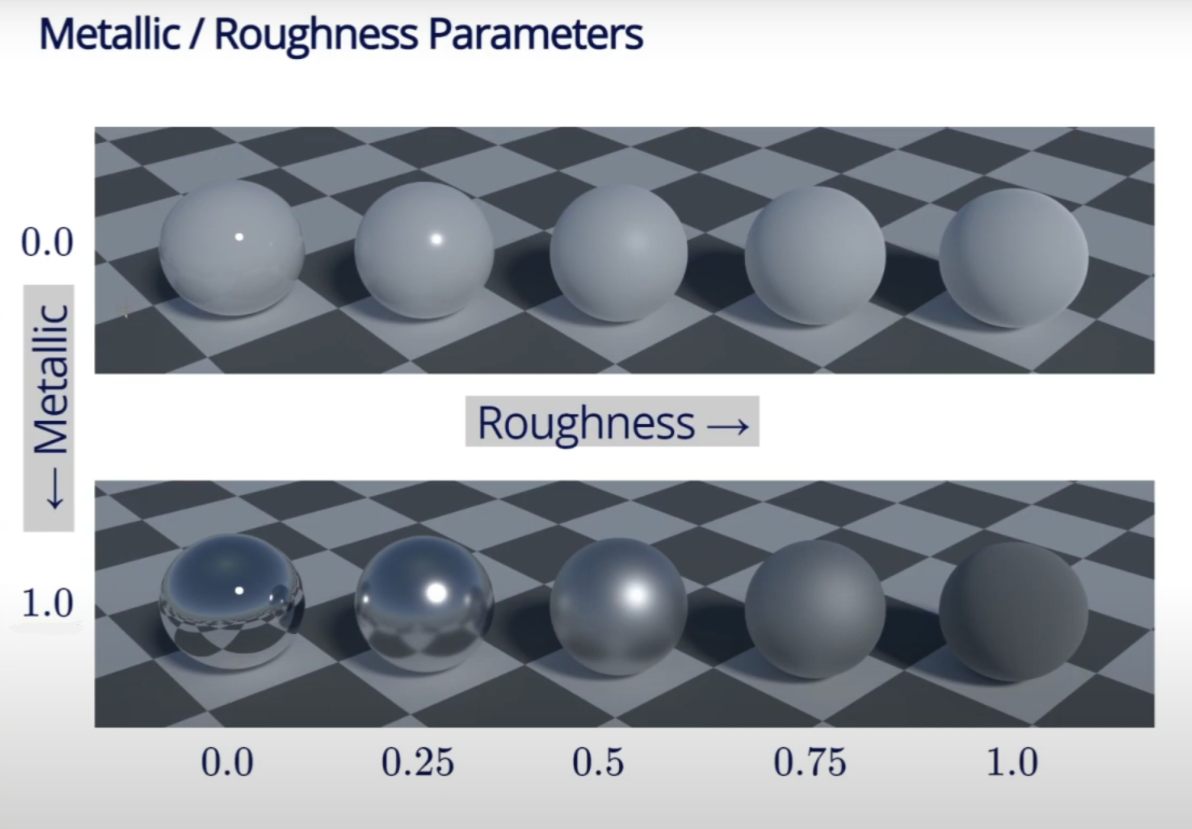
\includegraphics[scale=0.4]{Pictures/rough-metal.png}
  \caption{Металево-шорсткий підхід}
  \label{fig:RM}
\end{figure}

\par
Хоча модель Disney дозволяє використовувати дробові значення па\-ра\-мет\-ра \textit{metallic} (наприклад, $0.5$), фізично це не має сенсу, оскільки матеріал не може 
одночасно бути і металом, і діелектриком. Проте у практичних випадках, особливо при використанні текстур з обмеженою роздільною здатністю, у межах одного 
пікселя може міститися інформація про кілька матеріалів. У таких ситуаціях дробові значення \textit{metallic} інтерпретуються як середнє значення між різними типами 
матеріалів.

\par
Ще одним важливим параметром у моделі є \textbf{базовий колір} (\textit{base color}) рис. (\ref{fig:BC}). Це вектор з трьох компонентів (RGB), 
який відіграє різну роль за\-леж\-но від типу матеріалу.

\begin{itemize}
    \item Для \textbf{діелектриків} (неметалів) цей параметр визначає альбедо ма\-те\-ріа\-лу -- тобто частку світла, яка дифузно відбивається від поверхні. Значення кожної 
    компоненти RGB знаходиться в межах інтервалу $[0;1]$.
    
    \item Для \textbf{металів}, навпаки, \texit{base color} представляє значення коефіцієнта відбиття Френеля при нормальному падінні (Fresnel reflectance), яке 
    характеризує дзеркальну компоненту відбитого світла. Докладний розгляд закону Френеля буде подано у наступному підрозділі.
\end{itemize}

\begin{figure}[h]
  \centering
  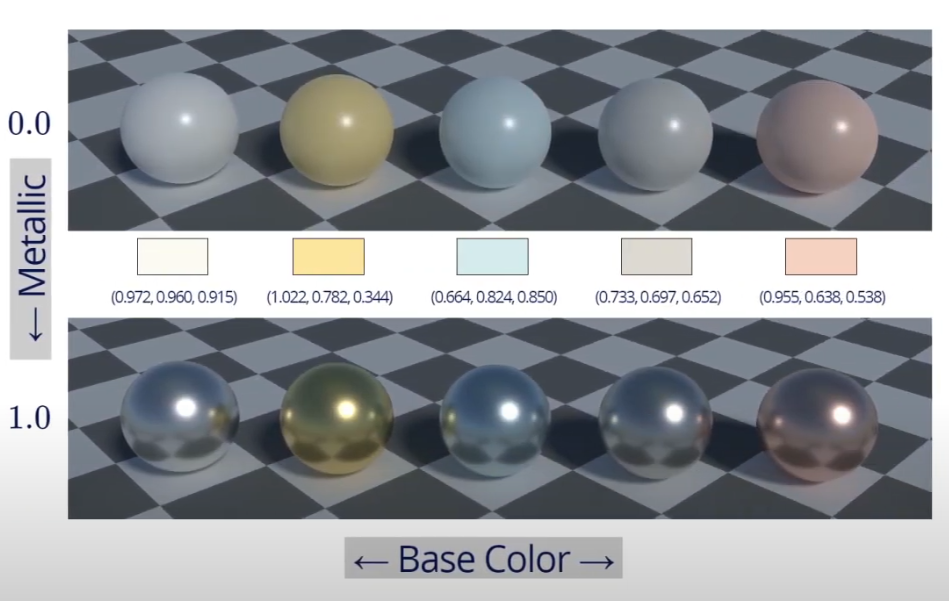
\includegraphics[scale=0.6]{Pictures/BaseColor.png}
  \caption{Базовий колір матеріалів}
  \label{fig:BC}
\end{figure}

Крім того, у моделі передбачено ще один параметр -- \textbf{відбивна здатність} (\textit{reflectance}) рис. (\ref{fig:Specular}), який застосовується лише для діелектричних матеріалів. 
Він також пов’язаний із законом Френеля, однак для неметалів. Цей параметр визначає інтенсивність дзеркальної компоненти відбиття (specular ref\-lec\-tion), 
притаманної діелектрикам.

На відміну від металів, де дзеркальне відбиття при нормальному падінні світла може досягати майже $100\%$, для діелектриків цей показник значно нижчий -- він 
зазвичай перебуває в межах від 0\% до 16\% залежно від матеріалу та кута падіння, та за для зручності ці межі відображають у відрізок $[0,1]$.

\begin{figure}[h]
  \centering
  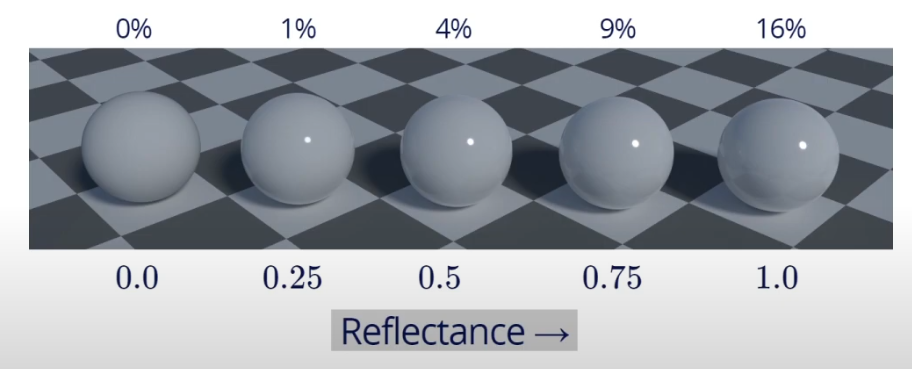
\includegraphics[scale=0.75]{Pictures/Specular.png}
  \caption{Відбивна здатність}
  \label{fig:Specular}
\end{figure}

\par
У рівнянні \ref{eq:RenderingEquation} BRDF виступає у ролі функці $f_r$. Так як BRDF належить до сімейства функцій,
точного вигляду вона немає. В даній квалфікаційній роботі розглядається Cook-Torrance BRDF модель, яка має такий вигляд:
\begin{equation}
\label{eq:BRDF}
f_r(\vec{v},\vec{l}) = \frac{\rho_d}{\pi} + \frac{\mathbf{F}(\vec{v},\vec{h})\cdot\mathbf{D}(\vec{h})\cdot\mathbf{G}(\vec{l},\vec{v})}{4 \cdot\langle \vec{n}, \vec{l}\rangle \cdot\langle \vec{n}, \vec{v}\rangle},
\end{equation}
де, $\vec{v}$ -- це вектор спостереження, тобто вектор у напрямку ока, $\vec{l}$ напрямок промення світла, $\vec{h}$ напівнапрямленний вектор, $\vec{n}$ нормаль поверхні та $\rho_d$ деяка константа.
Тут перший доданок виступає у ролі $f_d$, а другий у ролі $f_s$ рівності \ref{eq:BRDF_DS}. Окрім того, $\mathbf{F}(\vec{v},\vec{h})$ -- відбиття Френеля, $\mathbf{D}(\vec{h})$ -- функція
розподілу нормалей та $\mathbf{G}(\vec{l},\vec{v})$ -- геометричний фактор.

\subsection{Ефект Френеля}
 \setcounter{equation}{0}
 \setcounter{theorem}{0}

Один із ключових етапів побудови фізично коректної моделі відбиття світла полягає у врахуванні \textit{ефекту Френеля}, який описує залежність коефіцієнта 
відбиття від кута падіння світла та показників заломлення матеріалів на межі поділу середовищ.

\par
Ефект Френеля легко можна спостерігати в реальному житті. Наприклад, на рис.\ref{fig:FresnelLake} зображено озеро з абсолютно рівною поверхнею води; у нижній час\-ти\-ні чітко видно дно. 
Натомість у верхній частині видно лише відбиття. Така різниця пояснюється тим, що співвідношення між переданим і відбитим світ\-лом не є сталим: воно змінюється 
залежно від кута падіння променя та оп\-тич\-них властивостей (показників заломлення) матеріалів.

Коли ми дивимося у воду під прямим кутом, лише незначна частина світла відбивається, решта проходить крізь поверхню води, і ми бачимо дно. Проте зі збільшенням кута
 (наближенням до дотичного спостереження), частка відбитого світла зростає, а частка переданого -- зменшується. Тобто при малих кутах падіння спостерігається в основному 
 пропускання, а при великих -- відбиття.

 \begin{figure}[h]
  \centering
  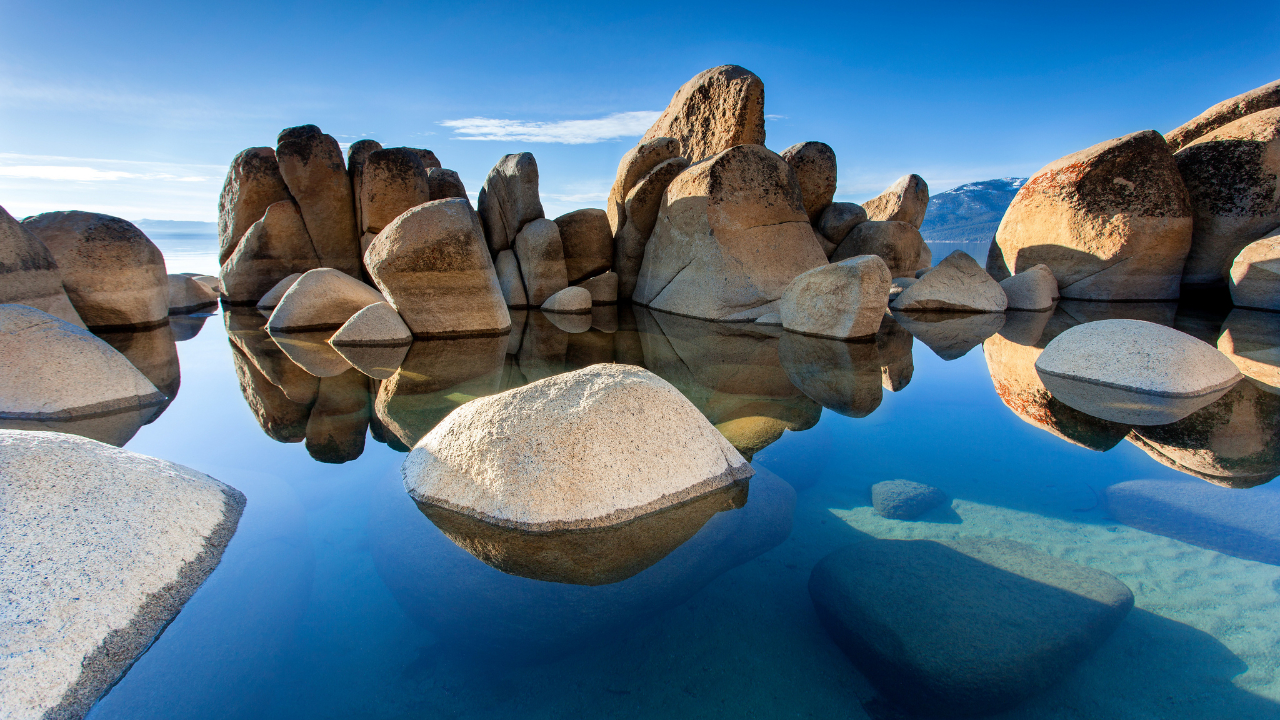
\includegraphics[scale=0.25]{Pictures/fresnelLake.jpg}
  \caption{Ефект Френеля в реальному житті}
  \label{fig:FresnelLake}
\end{figure}

\newpage
На рис. \ref{fig:Snells} зображено типову ситуацію взаємодії світла з поверхнею на межі двох середовищ. У випадку басейну це межа повітря 
(з показником заломлення $\eta_1$) і води (з більшим показником заломлення $\eta_2$). Кут падіння $\theta_1$ визначається відносно нормалі до поверхні. Закон 
відбиття стверджує, що кут між нормаллю та відбитим променем дорівнює $\theta_1$. Для заломленого (переданого) променя кут $\theta_2$ є меншим, оскільки світло 
переходить із менш густого середовища у густіше (тобто промені заломлюються у бік нормалі).

Цей зв’язок описується законом Снеліуса:
\begin{equation*}
    \eta_1 \sin \theta_1 = \eta_2 \sin \theta_2,
\end{equation*}
де $\eta_1$ та $\eta_2$ -- показники заломлення відповідних середовищ, $\theta_1$ -- кут падіння, а $\theta_2$ -- кут заломлення.


 \begin{figure}[h]
  \centering
  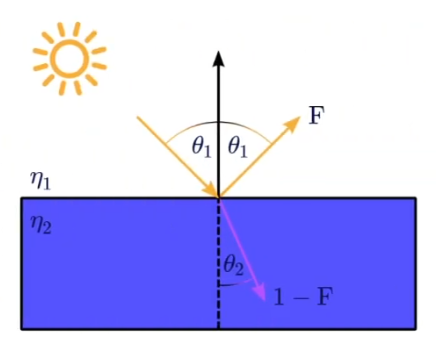
\includegraphics[scale=0.75]{Pictures/Snells.png}
  \caption{Заломлення світла}
  \label{fig:Snells}
\end{figure}

Знаючи $\eta_1$, $\eta_2$ та $\theta_1$, ми можемо обчислити $\theta_2$ і, у подальшому, розрахувати частку відбитого світла за допомогою рівнянь Френеля:
\begin{equation*}
F_{para} = \frac{\eta_2\cos\theta_1 - \eta_1\cos\theta_2}{\eta_2\cos\theta_1 + \eta_1\cos\theta_2};
\end{equation*}
\begin{equation*}
F_{pere} = \frac{\eta_2\cos\theta_2 - \eta_1\cos\theta_1}{\eta_2\cos\theta_2 + \eta_1\cos\theta_1};
\end{equation*}
\begin{equation}
\label{eq:fresnel}
F = \frac{1}{2}(F_{para} + F_{pere}).\quad
\end{equation}

Частка переданого світла визначається як:
\begin{equation*}
    T = 1 - R,
\end{equation*}
де $R$ -- коефіцієнт відбиття, який залежить від поляризації світла, кута падіння та оптичних властивостей матеріалів.
\paragraph{Відбиття Френеля для діелектриків та металів.}

\par 
Світлові фотони при взаємодії з поверхнею можуть бути відбитими із певними йомовірностями, які напряму залежать від кута падіння. Для діе\-ле\-кт\-ри\-ків, відбита частина світла розсіюється мікрофасетками поверхні, що мак\-ро\-ско\-піч\-но формує дзеркальну складову відбиття. Передана частина зазнає внут\-ріш\-ніх 
 розсіянь, частково поглинається і випромінюється у випадкових напрямках. Це створює дифузну складову.
Чим більше світла відбивається на поверхні, тим менше його проникає всередину, а отже, дифузна складова стає слабшою. Оскільки ймовірність поглинання світла 
залежить від довжини хвилі, то дифузна частина є кольоровою. Натомість дзеркальна складова зазвичай є некольоровою для діелектриків.


\par
Для металів ситуація інакша: передана частина повністю поглинається, тому дифузна складова відсутня. Натомість дзеркальна складова є кольоровою, оскільки залежить
 від довжини хвилі. Це пояснює, чому метали мають ха\-рак\-тер\-не забарвлення у дзеркальних відбиттях.

 \par
Для перпендикулярного падіння ($\theta_1 = 0^\circ$), рівняння Френеля значно спрощуються. Якщо припустити, що $\eta_1 = 1$ (повітря або вакуум), а $\eta_2 = 1.5$ 
(наприклад, скло), то за формулою \ref{eq:fresnel} можна обчислити значення $F_0 \approx 0.04$, тобто $4\%$ світла буде відбито, а 96\% -- пропущено.

\begin{equation*}
    F_0 = \left( \frac{\eta_2 - \eta_1}{\eta_2 + \eta_1} \right)^2.
\end{equation*}

\par 
У мікрофасетній моделі поверхня складається з великої кількості кри\-хіт\-них ідеально плоских дзеркал. Через це для розрахунку відбиття Френеля ми використовуємо не кут між 
вхідним променем та нормаллю поверхні, а кут між напрямком огляду (або світла) і вектором півшляху (halfway vector). У данному випадку
вектор півшляху використовується як нормаль мікрофасеток через те, що нас цікавить частина світла яка відбивається у напрямок спостерігача:

\begin{equation}
    \cos \theta = \langle\vec{v}, \vec{h}\rangle.
\end{equation}

Тому саме цей кут $\theta$ використовується у рівняннях Френеля в мікрофасетній BRDF-моделі, запропонованій Куком і Торренсом (Cook \& Torrance, 1982) \cite{cook1982reflectance}, та
ефект Френеля обчислюється наступним чином:
\begin{equation}
  F_{Cook-Torrance}(\vec{v},\vec{h}) = \frac{1}{2}(\frac{g - c}{g + c})^2(1 + (\frac{c(g+c)-1}{c(g-c)+1})^2),
\end{equation}
де $c = \langle\vec{v},\vec{h}\rangle$ та $g = \sqrt{\eta_2^2+c^2-1}$.
Незважаючи на відсутність тригонометричних функцій, ці обчислення є дорогими. Щоб зменшити обчислювальні витрати, часто використовують \textit{апроксимацію 
Шліка (aнгл. Schlick's approximation)}:

\begin{equation}
    F_{Schlick}(\theta) = F_0 + (1 - F_0)(1 - \cos \theta)^5.
\end{equation}

Ця формула дозволяє швидко наближати поведінку функції Френеля без втрати надто великої точності.
 Як показано на рис. \ref{fig:Schlick}, при $\theta = 0^\circ$ вона точно дає $F = F_0$, а при $\theta = 90^\circ$ -- $F = 1$. 
 У проміжних кутах апроксимація лише незначно відхиляється від точного розв’язку.
 \begin{figure}[h]
  \centering
  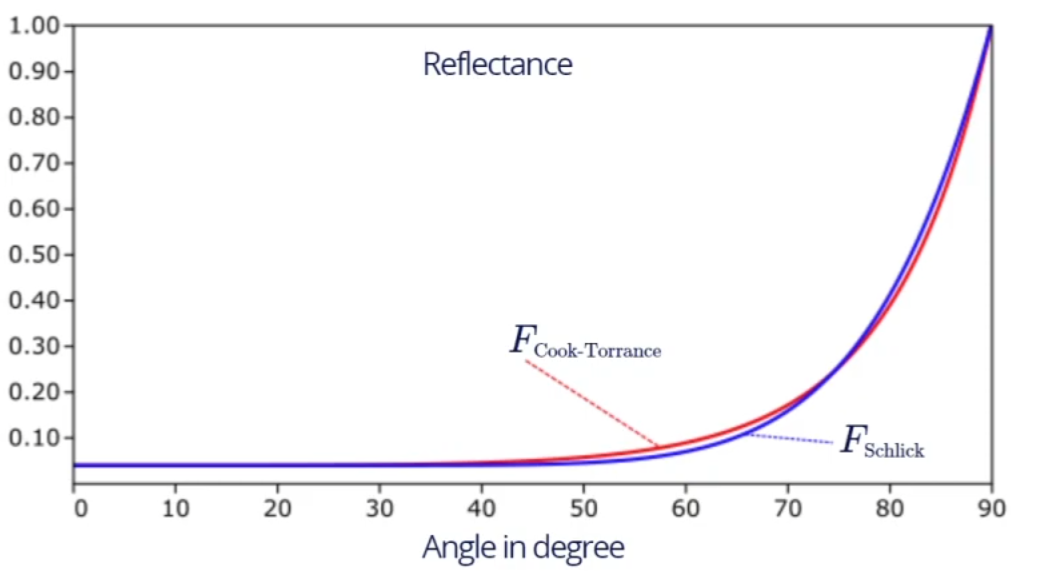
\includegraphics[scale=0.55]{Pictures/Shlick.png}
  \caption{Порівняння апроксимацію Шліка}
  \label{fig:Schlick}
\end{figure}

Цей підхід широко використовується у реальному часі (наприклад, у PBR-шейдерах), забезпечуючи добрий баланс між точністю і швидкодією.

\subsection{Функція розподілу нормалей}\\

\par
Як вже зазначалося раніше, поверхня фізичного матеріалу має мікроскопічну шорсткість, яка складається з безлічі мікрофасетів із власними мікронормалями. 
Ця мікроструктура відіграє ключову роль у формуванні зовнішнього вигляду поверхні під час взаємодії зі світлом.

Розподіл таких мікронормалей описується за допомогою функції розподілу нормалей (NDF, \textit{Normal Distribution Function}). Вона є складовою частиною 
двонапрямної функції розподілу відбиття, яка визначає, як світло від\-би\-ва\-єть\-ся з поверхні y 
заданому напрямку.

BRDF формалізує кількість енергії, що відбивається від поверхні в напрямку спостерігача від одного променя вхідного світла. Вона є зваженою величиною, оскільки 
враховує NDF, яка насправді є функцією розподілу ймовірностей (PDF, \textit{Probability Distribution Function}) для напрямків мікронормалей.

У випадку ідеально гладкої, полірованої поверхні всі мікрофасети орієнтовані в одному напрямку -- відповідно до макроскопічної нормалі поверхні. Натомість 
при більш шорсткій поверхні орієнтації мікрофасетів статистично розподілені навколо цієї нормалі. Відповідно, відбиття світла також розсіюється навколо ідеального
 дзеркального напрямку. Із зростанням шорсткості поверхні ступінь цього розсіювання збільшується рис. (\ref{fig:NDF}).

  \begin{figure}[h]
  \centering
  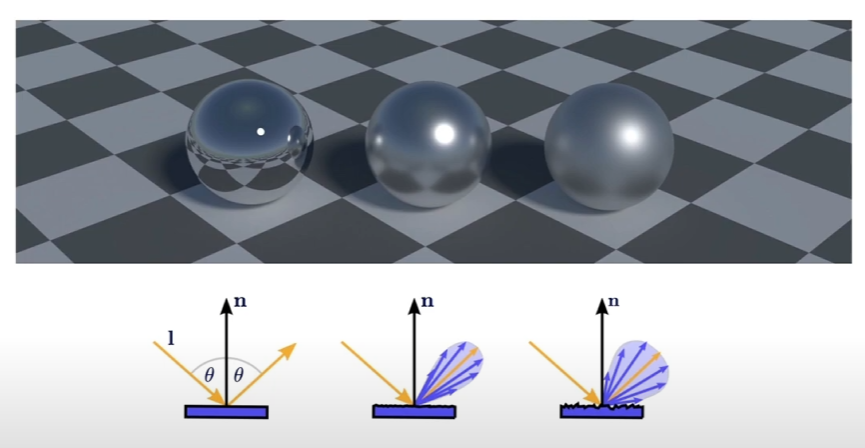
\includegraphics[scale=1]{Pictures/NDF.png}
  \caption{Вплив функції розподілу нормалей}
  \label{fig:NDF}
\end{figure}

Таким чином, функція розподілу нормалей NDF визначає, наскільки вірогідною є наявність мікрофасета певної орієнтації в даній точці поверхні. Ця ймовірність 
безпосередньо впливає на вигляд відбитого світла, а отже -- і на візуальне сприйняття матеріалу.
\par 
  У моделі Cook-Torrance, NDF розраховується за формулою:
\begin{equation}
  D_{GGX}(\vec{h})=\frac{\alpha^2}{\pi(\langle\vec{n},\vec{h}\rangle^2(\alpha^2-1)+1)^2},
\end{equation}
де $\alpha = r_p^2$, а $r_p$ -- шорсткість матеріалу та приймає значення на відрізку $[0,1]$.

\subsection{Геометричний фактор}\\

\par
Останнім елементом мікрофасетної моделі є геометричний фактор, який враховує ефекти затінення (\textit{shadowing}) та перекриття (\textit{masking}) 
мікрофасетів. Ці ефекти виникають залежно від напрямку падіння світла та напрямку огляду спостерігача.

У роботі Кука і Торренса, передбачається, що мікрофасети мають форму літери V. 
На основі цієї моделі було виведено геометричний термін, який описує ймовірність того, що світло буде заблоковане іншими мікрофасетами 
або не зможе відбитися в напрямку спостерігача, обчислюється він наступним чином:
\begin{equation*}
  G_{Cook-Torrance}(\vec{l},\vec{v}) = min(1, \frac{2\langle\vec{n},\vec{h}\rangle\langle\vec{n},\vec{v}\rangle}
  {\langle\vec{v},\vec{h}\rangle},
  \frac{2\langle\vec{n},\vec{h}\rangle\langle\vec{n},\vec{l}\rangle}
  {\langle\vec{v},\vec{h}\rangle}).
\end{equation*}

Залежно від конфігурації, можливі три випадки: відсутність перешкод, \linebreak ефект перекриття при поглядових кутах під ковзаючим кутом, 
або затінення при падінні світла під аналогічним кутом (див. рис. \ref{fig:GeometryTerm}).Для нульового значення шорсткості (ідеально гладка поверхня) геометричний фактор дорівнює 1, 
тобто не впливає на результат. Зі збільшенням шорсткості значення геометричного фактору зменшується, 
що відповідає фізично очікуваному ефекту -- зростанню ймовірності перекриття і затінення мікрофасетів.

\begin{figure}[h]
  \centering
  \hspace*{-1.7cm} % або -0.1cm, -2mm тощо
  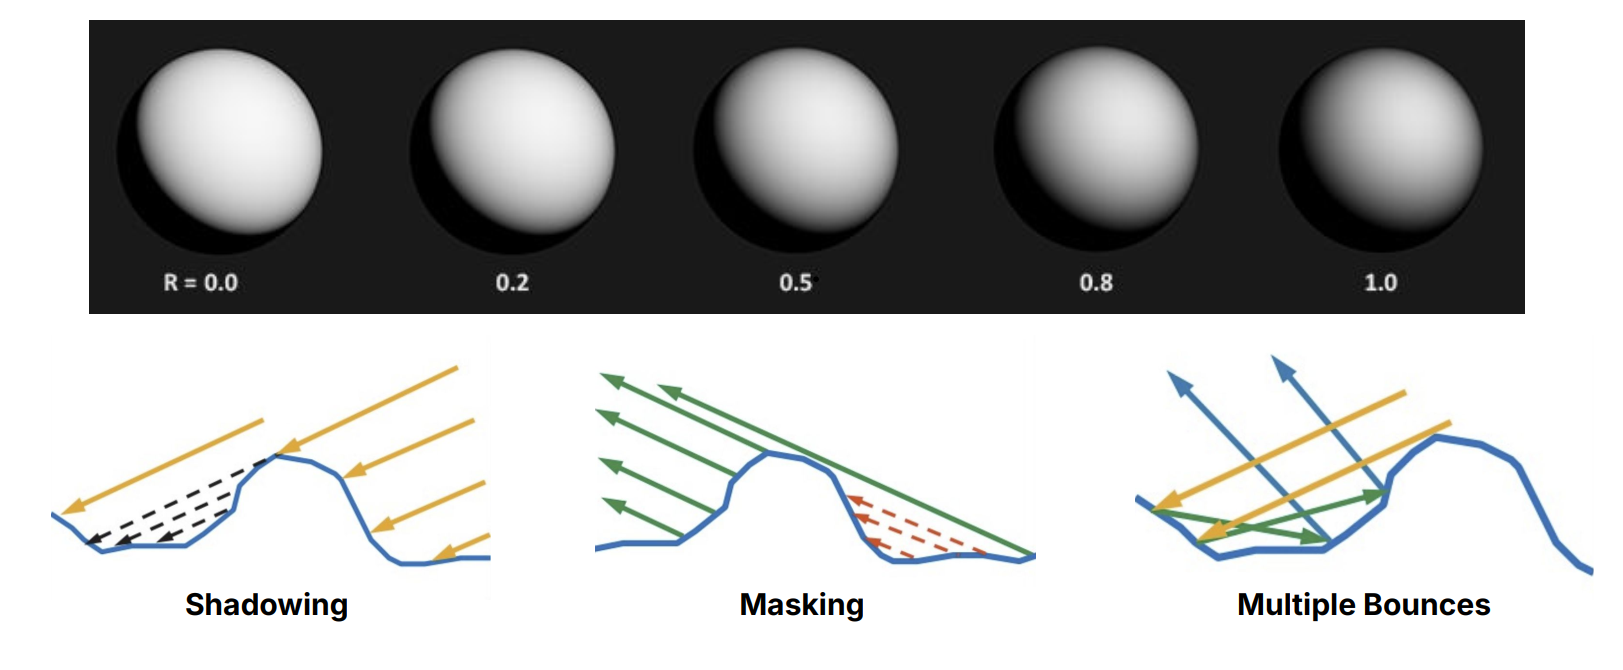
\includegraphics[scale=0.65]{Pictures/GeometryTerm.png}
  \caption{Вплив геометричного фактору}
  \label{fig:GeometryTerm}
\end{figure}



Іншу відому модель геометричного фактору запропонував Б.~Дж.~Сміт\linebreak (B.~J.~Smith) у 1967 році. 
У ній геометричний фактор обчислюється як добуток двох однакових функцій $G_1$, які розраховуються окремо для напрямку світла та напрямку огляду:

\[
G(l, v) = G_1(l) \cdot G_1(v).
\]

За функцію $G_1$ було обрано:
\begin{equation*}
  G(\vec{v}) = \frac{\sqrt{2}}{\sqrt{1 + \frac{\alpha(1-\langle\vec{n},\vec{v}\rangle)}{\langle\vec{n},\vec{v}\rangle}}}.
\end{equation*}
Таким чином, остаточне аналітичне представлення геометричного фактору, що враховує вплив мікроструктури поверхні на явища екранування та за\-ті\-нен\-ня, набуває наступного вигляду:

\begin{equation}
  \label{eq:GT}
G = \frac{2}{\sqrt{1 + \frac{\alpha(1-\langle\vec{n},\vec{v}\rangle)}{\langle\vec{n},\vec{v}\rangle}}
\sqrt{1 + \frac{\alpha(1-\langle\vec{n},\vec{l}\rangle)}{\langle\vec{n},\vec{l}\rangle}}}.
\end{equation}

Цей вираз є кульмінацією теоретичного узагальнення мікрофасетної геометрії, що водночас 
враховує складні взаємодії світлового потоку з текстурною нерівністю реальних поверхонь. Його 
застосування забезпечує фізично коректне моделювання поведінки світла на мікроскопічному рівні, що 
є критично важливим для створення фотореалістичних комп’ютерних зображень.

\par Такий підхід дозволяє точно моделювати як дифузні, так і дзеркальні відбиття, залежно від
оптичних характеристик матеріалу, зокрема показника заломлення, ступеня шорсткості та кута падіння 
світла. Завдяки цьому, система освітлення здатна відтворювати складну взаємодію світла з матеріалом -- 
від блискучих металів до матових діелектриків -- з урахуванням енергозбереження та фізичної правдоподібності.

\par У практичній реалізації мікрофасетної моделі критичним є вибір функції розподілу нормалей 
поверхні (NDF), таких як GGX або Beckmann, які визначають імовірнісний розподіл мікрофасеток по орієнтаціях. 
Це, в поєднанні з геометричними термінами самозатінення (G) та френелівськими коефіцієнтами (F), утворює 
повноцінну BRDF-модель (наприклад, Кука-Торренса), що дозволяє інтегрувати фізику світлових явищ 
у рендерінг-алгоритми сучасних графічних рушіїв.

\par Саме через ці характеристики мікрофасетна модель виступає основою у більшості сучасних 
технік фізично коректного рендерингу (PBR) і є фундаментом для багатьох подальших удосконалень, 
включаючи імплементацію попередньо обчислених таблиць (LUT), вибір за значимістю (англ. importance sampling), а також 
застосування моделей освітлення на основі оточення (IBL), що в сукупності дозволяє досягати високого 
візуального реалізму при збереженні продуктивності.
